\chapter{Mondiale verandering en de biosfeer}\label{ch:b2:global-change}

Tussen 1851 en 1858 doorkruiste Henry Thoreau de bossen en weiden rond
Concord, Massachusetts, en noteerde hij voor zo'n vijfhonderd planten de dag
waarop ze voor het eerst bloeiden. Anderhalve eeuw later gingen botanici met
zijn aantekenboekjes terug naar dezelfde plekken. De blauwe bosbes die Thoreau
op 11 mei zag opengaan, gaat nu op 12 april open; de hele flora bloeit
gemiddeld tien dagen vroeger dan in zijn tijd, gelijk op met een lente die
\qty{2.4}{\celsius} warmer is; en een kwart van zijn soorten is uit Concord
verdwenen --- niet willekeurig, maar die waarvan de bloei de temperatuur niet
kon volgen. De vorige hoofdstukken gaven het mechanisme: de kringlopen
van \cref{ch:b2:biogeochemical-cycles}, de selectie en drift van
\cref{ch:b2:population-genetics}, de concurrentie en soortvorming
van \cref{ch:b2:speciation}, de \omterm{def:b2:living-soil:soil}{bodems} van \cref{ch:b2:living-soil}.
Dit hoofdstuk zet een getal op wat er met levende wezens gebeurt nu één soort
de chemie van de lucht en de zee verandert: hoeveel opwarming per ton koolstof,
hoeveel dagen lente per graad, hoeveel meter bergop, hoeveel zuur in de zee,
hoeveel soorten per verloren hectare --- en wat de getallen zeggen over de
komende eeuw.

\section{De fysische verandering}

\begin{proposition}[Opwarming is evenredig met de cumulatieve uitstoot]\label{prop:b2:global-change:tcre}
\index{opwarming van de aarde}\index{cumulatieve uitstoot}\index{koolstofbudget}\index{broeikaseffect}
Koolstofdioxide absorbeert het infrarood dat de grond uitstraalt en stuurt een
deel ervan terug; meer \ensuremath{\mathrm{CO_2}} betekent een warmer oppervlak, met
ongeveer \qty{3}{\celsius} per verdubbeling zodra de oceanen zijn bijgebeend
(de \emph{klimaatgevoeligheid}). Omdat de temperatuurrespons op
\ensuremath{\mathrm{CO_2}} logaritmisch is in de concentratie, terwijl de \omterm{prop:b2:biogeochemical-cycles:carbon}{atmosferische
fractie} van de uitstoot daalt naarmate de concentratie stijgt, heffen de twee
krommingen elkaar bijna op, en is de wereldgemiddelde opwarming in goede
benadering \emph{lineair in de cumulatieve hoeveelheid uitgestoten
koolstof}, ongeacht de timing:
\[
\Delta T \approx \lambda\,C_{\text{cum}}, \qquad \lambda \approx
\qty{1.65}{\celsius} \text{ per } \qty{1000}{GtC}
\]
(\qty{0.45}{\celsius} per \qty{1000}{Gt} \ensuremath{\mathrm{CO_2}}). De zo'n
\qty{700}{GtC} die sinds 1850 zijn uitgestoten, hebben de planeet
\qty{1.2}{\celsius} opgewarmd --- en de relatie geeft elk doel een
budget: \qty{1.5}{\celsius} laat in totaal ongeveer \qty{900}{GtC} toe,
\qty{200}{GtC} meer dan al is uitgestoten, twintig jaar in het
huidige tempo. De opwarming is ongelijk: twee keer het gemiddelde boven land
en drie keer in het Noordpoolgebied; 's nachts meer dan overdag; en ze komt
met de rest --- hevigere regen en langere droogtes, een zeespiegel
die \qty{4}{mm} per jaar stijgt, zee-ijs dat in de zomer een vijfde kleiner is,
en een oceaan die \qty{90}{\%} van de warmte en een kwart van de koolstof heeft
opgenomen.
\end{proposition}
\begin{proof}[Bewijsmateriaal]
De evenredigheid werd gevonden in klimaatmodellen van elke complexiteit en
bevestigd door de waargenomen reeks: de opwarming sinds 1850 uitgezet tegen
de \omterm{prop:b2:global-change:tcre}{cumulatieve uitstoot} geeft door de decennia heen een rechte lijn. Het
broeikaseffect zelf wordt vanuit een baan om de aarde gemeten: satellieten zien
het infrarood dat de aarde uitstraalt, met de absorptiebanden van
\ensuremath{\mathrm{CO_2}}, methaan en waterdamp eruit weggesneden, en die insnijding is
tussen 1970 en 2020 precies zoveel dieper geworden als de stijging van deze
gassen voorspelt. De isotopen en de dalende zuurstof van
\cref{ch:b2:biogeochemical-cycles} koppelen het extra
\ensuremath{\mathrm{CO_2}} aan fossiele brandstof.
\end{proof}

\begin{omfigure}
\begin{tikzpicture}
\begin{axis}[
  width=0.88\linewidth, height=5.6cm,
  axis x line=bottom, axis y line=left,
  xmin=1845, xmax=2030, ymin=-0.3, ymax=1.5,
  xlabel={decennium}, ylabel={opwarming (\unit{\celsius}) sinds 1850--1900},
  xlabel style={font=\small, at={(axis description cs:0.5,-0.13)}, anchor=north},
  ylabel style={font=\small},
  tick label style={font=\small}, xtick={1850,1900,1950,2000}, ytick={0,0.5,1,1.5},
  scaled x ticks=false, x tick label style={/pgf/number format/1000 sep=},
  clip=false,
]
\addplot[ybar, bar width=7pt, fill=omThm!50, draw=omThm] coordinates {
(1855,0.00) (1865,-0.04) (1875,0.02) (1885,-0.06) (1895,-0.02) (1905,-0.10) (1915,-0.06) (1925,0.05) (1935,0.15) (1945,0.25) (1955,0.15) (1965,0.15) (1975,0.18) (1985,0.40) (1995,0.55) (2005,0.78) (2015,1.02) (2023,1.28)};
\node[font=\scriptsize, anchor=west, align=left] at (axis cs:1850,1.2) {elke staaf: het gemiddelde van een decennium; de laatste 2020--2024\\ \qty{700}{GtC} uitgestoten, $\qty{1.65}{\celsius}/\qty{1000}{GtC}$: \qty{1.2}{\celsius}};
\end{axis}
\end{tikzpicture}

{\small Wereldgemiddelde oppervlaktetemperatuur per decennium, ten opzichte van
de tweede helft van de negentiende eeuw. Elk van de laatste vier decennia
vestigde een record, en de stijging sinds 1970 bedraagt \qty{0.2}{\celsius} per
decennium.}
\end{omfigure}

\section{De kalender: fenologie}

\begin{theorem}[Graaddagen en het vervroegen van de lente]\label{thm:b2:global-change:phenology}
\index{fenologie}\index{graaddagen}\index{thermische tijd}\index{fenologische ontkoppeling}
Veel gebeurtenissen in het leven van planten en ectotherme dieren ---
knopuitloop, bloei, het uitkomen van eieren, emergentie --- vinden plaats
wanneer de opgestapelde \emph{\omterm{thm:b2:global-change:phenology}{thermische tijd}} sinds een begindatum, de som van
de dagtemperaturen boven een basis $T_b$ (\emph{graaddagen}), een
vast totaal $K$ bereikt. Als de lentetemperatuur lineair stijgt, $T(t) = T_b
+ b\,(t - t_0)$ met $b$ graden per dag vanaf de dag $t_0$ waarop ze
de basis overschrijdt, vindt de gebeurtenis plaats op
\[
t^{*} = t_0 + \sqrt{2K/b},
\]
en een gelijkmatige opwarming met $\Delta T$ vervroegt de dag van overschrijding
met $\Delta T/b$, en de gebeurtenis mee: met $b \approx
\qty{0.1}{\celsius}$ per dag \emph{ongeveer tien dagen vroeger per
graad}. Soorten verschillen in $T_b$ en $K$, en in de vraag of ze ook de
daglengte gebruiken, die door opwarming niet verandert --- zodat de leden van
een voedselketen met verschillende snelheden vervroegen en hun timing
uiteenvalt: een \emph{\omterm{thm:b2:global-change:phenology}{fenologische ontkoppeling}} tussen de rups en
de vogel die er zijn kuikens mee moet voeren.
\end{theorem}
\begin{proof}
Graaddagen vanaf $t_0$: $\int_{t_0}^{t}(T - T_b)\,\mathrm{d}t' =
b\,(t - t_0)^{2}/2$, gelijk aan $K$ wanneer $t - t_0 = \sqrt{2K/b}$.
Opwarming met $\Delta T$ vervangt $T$ door $T + \Delta T$: de basis wordt
$\Delta T/b$ dagen eerder overschreden, en de opstapeling, vanaf die dag
identiek, is $\Delta T/b$ dagen eerder voltooid. (Als de opwarming ook $b$
steiler maakt, wordt het interval $\sqrt{2K/b}$ eveneens korter.) Een soort
die zich op de daglengte richt, houdt haar datum; een soort die zich op
graaddagen richt, verschuift; de kloof tussen hen groeit met $\Delta T/b$.
\end{proof}
\begin{proof}[Bewijsmateriaal]
De flora van Thoreau in Concord, en de aantekeningen van de familie Marsham
over zevenentwintig lentetekens in Norfolk, bijgehouden van 1736 tot 1947,
tonen allebei een vervroeging van bloei en bladontplooiing met
\qtyrange{3}{6}{d} per graad lenteopwarming. De kersenbloesem van Kyoto,
sinds de negende eeuw gedateerd in hofdagboeken, bleef duizend jaar rond
half april en is sinds 1900 naar begin april verschoven, met de
vroegste data ooit in de jaren 2020. In Nederland bereiken de rupsen van de
eik nu twee weken vroeger hun piek dan in 1985; de koolmees, die zich op
dezelfde warmte richt, heeft gelijke tred gehouden, maar de bonte
vliegenvanger, die zijn trek vanuit Afrika op de daglengte afstemt, komt aan
zoals vroeger en vindt de piek voorbij --- zijn populaties zijn met
\qty{90}{\%} gedaald waar de ontkoppeling het grootst is (Both en
collega's, 2006).
\end{proof}

\begin{omfigure}
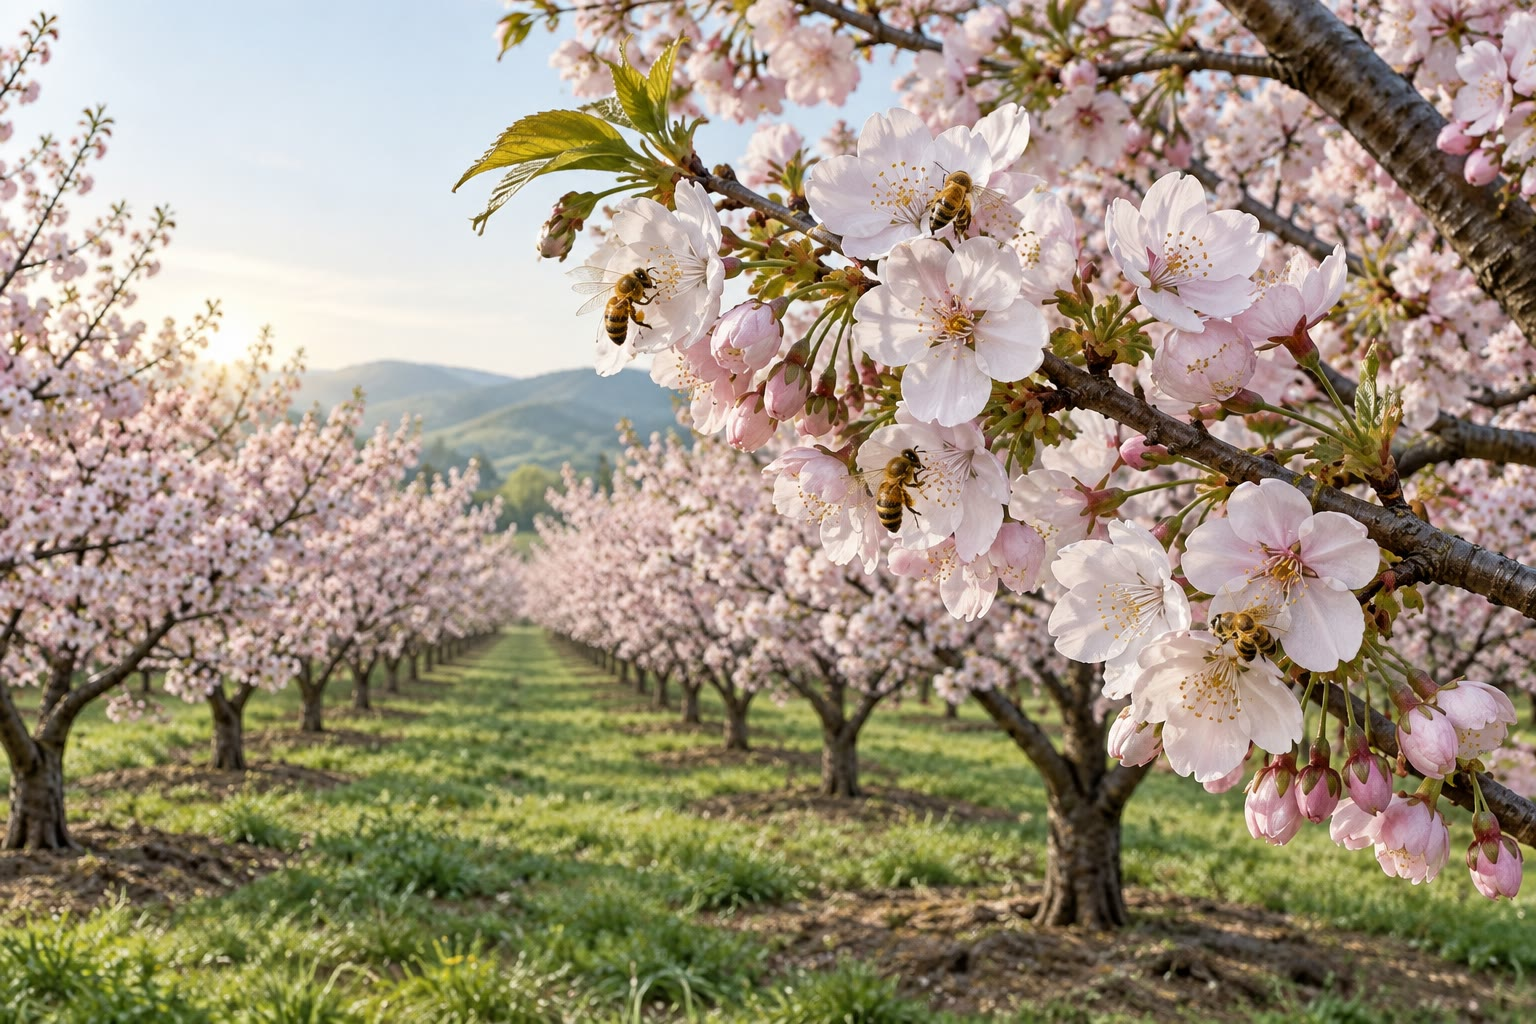
\includegraphics[width=0.62\linewidth]{images/book4/ai/b4-27-phenology-cherry.jpg}

{\small Een kersenboomgaard in bloei. De kersenbomen van Kyoto, al twaalf
eeuwen in dagboeken gedateerd, gaan nu vroeger open dan in enig jaar
vóór 1900 --- en de bijen die ze bestuiven, moeten op dezelfde dag vliegen.}
\end{omfigure}

\begin{omfigure}
\begin{tikzpicture}
\begin{axis}[
  width=0.74\linewidth, height=5.4cm,
  axis x line=bottom, axis y line=left,
  xmin=0, xmax=100, ymin=0, ymax=14,
  xlabel={dagen vanaf 1 maart}, ylabel={daggemiddelde temperatuur (\unit{\celsius})},
  xlabel style={font=\small, at={(axis description cs:0.5,-0.13)}, anchor=north},
  ylabel style={font=\small},
  tick label style={font=\small}, xtick={0,20,40,60,80,100},
  legend style={font=\scriptsize, at={(0.03,0.97)}, anchor=north west, draw=none},
  clip=false,
]
\addplot[very thick, omDef, domain=0:100, samples=2] {2 + 0.1*x};
\addlegendentry{lente vóór de opwarming}
\addplot[very thick, omThm, domain=0:100, samples=2] {3 + 0.1*x};
\addlegendentry{lente \qty{1}{\celsius} warmer}
\draw[dashed, gray] (axis cs:0,5) -- (axis cs:100,5); \node[font=\scriptsize, anchor=south east] at (axis cs:100,5) {basistemperatuur $T_b = \qty{5}{\celsius}$};
\fill[omDef, opacity=0.15] (axis cs:30,5) -- (axis cs:93,5) -- (axis cs:93,11.3) -- cycle;
\fill[omThm, opacity=0.15] (axis cs:20,5) -- (axis cs:83,5) -- (axis cs:83,11.3) -- cycle;
\draw[<->, thick] (axis cs:83,1.6) -- (axis cs:93,1.6); \node[font=\scriptsize, anchor=south] at (axis cs:88,1.8) {10 dagen};
\draw[dotted] (axis cs:93,0) -- (axis cs:93,5); \draw[dotted] (axis cs:83,0) -- (axis cs:83,5);
\node[font=\scriptsize, anchor=south, align=center] at (axis cs:62,11.4) {$K = 200$ graaddagen\\ (gearceerde oppervlakken)};
\end{axis}
\end{tikzpicture}

{\small Graaddagen. De gebeurtenis vindt plaats wanneer het gearceerde oppervlak
tussen de temperatuurlijn en de basis $K$ bereikt; een lente die één
graad warmer is, overschrijdt de basis tien dagen eerder en voltooit de
som tien dagen eerder.}
\end{omfigure}

\section{De kaart: areaalverschuivingen}

\begin{proposition}[Isothermen verschuiven, en soorten volgen]\label{prop:b2:global-change:range}
\index{areaalverschuiving}\index{klimaatsnelheid}\index{verticale temperatuurgradiënt}
De temperatuur daalt met ongeveer \qty{6.5}{\celsius} per kilometer
hoogte en met ongeveer \qty{0.65}{\celsius} per honderd kilometer
breedtegraad in de gematigde zone; een opwarming van \qty{1}{\celsius}
verschuift elke isotherm dus ongeveer \qty{150}{m} bergop en
\qty{150}{km} naar de pool. Soorten waarvan de grenzen door de temperatuur
worden bepaald, verschuiven mee met hun isotherm als ze kunnen: het gemiddelde
van honderden bestudeerde soorten is sinds 1970 per decennium \qty{11}{m}
bergop en \qty{17}{km} naar de pool geschoven, met de snelheid van de
isothermen, en de snelste --- mobiel, generalist, kortlevend --- lopen ze
voorbij, terwijl bomen, waarvan de zaden enkele meters per jaar reizen, en
soorten die al op de top of bij de pool zitten, niet kunnen volgen: de top van
een berg kan nergens heen, en elke graad opwarming neemt de hoogste
\qty{150}{m} van elk areaal weg. Mariene soorten, zonder barrières en met
scherpere thermische grenzen, verschuiven het snelst, tientallen kilometers per
decennium; de kabeljauw, de makreel en met hen de visserij zijn over hele zeeën
naar het noorden getrokken. De bovengrens van een areaal schuift op, de
ondergrens trekt terug naarmate het daar warmer wordt en er nieuwe
concurrenten van beneden aankomen, en de gemeenschap op elke plek wordt
opnieuw samengesteld uit soorten die elkaar nooit hebben ontmoet.
\end{proposition}
\begin{proof}[Bewijsmateriaal]
Parmesan (1996) inventariseerde opnieuw de Amerikaanse dambordvlinder van Edith
in zijn areaal in het westen van Noord-Amerika: populaties aan de
zuidrand en op lage hoogte waren uitgestorven, die aan de noordrand
en op grote hoogte bloeiden, en het hele areaal was
\qty{92}{km} naar het noorden en \qty{124}{m} omhoog geschoven --- de eerste
soort waarvan werd aangetoond dat ze de isothermen had gevolgd. Lenoir en
collega's (2008) vergeleken inventarisaties van bosplanten van 1905--1985 met
die van 1986--2005 in de Franse gebergten: de optimale hoogte van 171 soorten
was per decennium \qty{29}{m} gestegen. Chen en collega's (2011) vonden over
tweeduizend soorten verschuivingen die twee tot drie keer sneller waren dan
eerdere schattingen, en evenredig met de lokale opwarming.
\end{proof}

\begin{omfigure}
\begin{tikzpicture}[every node/.style={font=\scriptsize}, >=stealth]
  \fill[gray!25] (0,0) -- (3.5,4.2) -- (7,0) -- cycle;
  \draw[thick] (0,0) -- (3.5,4.2) -- (7,0);
  \foreach \y/\lab in {1.0/{\qty{12}{\celsius}}, 2.2/{\qty{8}{\celsius}}, 3.4/{\qty{4}{\celsius}}} { \draw[omDef, thick] ({\y/1.2},\y) -- ({7-\y/1.2},\y) node[right] {\lab}; }
  \foreach \y in {1.15,2.35,3.55} { \draw[omThm, thick, dashed] ({\y/1.2},\y) -- ({7-\y/1.2},\y); }
  \node[omThm, anchor=west, align=left] at (7.6,3.7) {gestippeld: dezelfde isothermen\\ na \qty{1}{\celsius} opwarming,\\ \qty{150}{m} hoger};
  \fill[omProp!50] (0.83,1.0) -- (6.17,1.0) -- (5.17,2.2) -- (1.83,2.2) -- cycle;
  \node[align=center] at (3.5,1.6) {de band van een soort,\\ \qtyrange{1000}{1200}{m}};
  \draw[->, thick, omExo!80!black] (1.1,2.2) -- (1.1,2.9); \node[omExo!80!black, anchor=east, align=right] at (0.95,2.55) {de band schuift op\\ en krimpt};
  \node[anchor=north] at (3.5,-0.1) {een berg: het oppervlak krimpt met de hoogte, en boven de top is er niets hogers};
\end{tikzpicture}

{\small Een \omterm{prop:b2:global-change:range}{areaalverschuiving} op een berg. Elke graad tilt de
isothermen \qty{150}{m} op; een soort volgt haar band naar boven, naar een
kleiner oppervlak, en een band die al op de top ligt, gaat verloren.}
\end{omfigure}

\section{De zee: verzuring en warmte}

\begin{theorem}[Verzuring]\label{thm:b2:global-change:acid}
\index{oceaanverzuring}\index{carbonaatsysteem}\index{verzadigingstoestand}\index{koraalverbleking}
Koolstofdioxide dat in zeewater oplost, vormt koolzuur, dat
dissocieert: $\ensuremath{\mathrm{CO_2}} + \ensuremath{\mathrm{H_2O}} \rightleftharpoons \ensuremath{\mathrm{H^{+}}} +
\ensuremath{\mathrm{HCO_3^{-}}}$, met $[\ensuremath{\mathrm{H^{+}}}][\ensuremath{\mathrm{HCO_3^{-}}}]/[\ensuremath{\mathrm{CO_2}}] = K_1$.
Bicarbonaat is de grootste koolstofvoorraad van de oceaan en wordt door de
alkaliniteit vrijwel constant gehouden, zodat
\[
[\ensuremath{\mathrm{H^{+}}}] \propto p_{\ensuremath{\mathrm{CO_2}}}, \qquad
\Delta\mathrm{pH} \approx -\log_{10}\frac{p_{\ensuremath{\mathrm{CO_2}}}}{p_0}
\]
--- nauwkeuriger $-0.9\log_{10}$ van de verhouding, omdat bicarbonaat
een beetje stijgt. Van 280 tot \qty{420}{ppm} is de pH aan het oppervlak
met $0.15$ gedaald, van $8.2$ tot $8.05$: een toename van de waterstofionen met
\qty{40}{\%}; bij \qty{800}{ppm} zou hij met $0.4$ dalen. De extra
waterstofionen verbruiken carbonaat, $\ensuremath{\mathrm{H^{+}}} + \ensuremath{\mathrm{CO_3^{2-}}} \to \ensuremath{\mathrm{HCO_3^{-}}}$, en
de \emph{\omterm{thm:b2:global-change:acid}{verzadigingstoestand}} $\Omega$ van calciumcarbonaat ---
het product van de calcium- en carbonaatconcentraties gedeeld door het
oplosbaarheidsproduct --- daalt evenredig: schelpen en skeletten
van aragoniet (koralen, pteropoden) vormen zich gemakkelijk bij $\Omega > 3$,
moeizaam rond 1, en lossen daaronder op; het tropische oppervlaktewater,
met $\Omega \approx 4$ vóór de industrie en 3 nu, bereikt 2 bij
\qty{560}{ppm}, en het koude, \ensuremath{\mathrm{CO_2}}-rijke oppervlaktewater
van de poolgebieden bereikt als eerste 1.
\end{theorem}
\begin{proof}
Uit het evenwicht volgt $[\ensuremath{\mathrm{H^{+}}}] = K_1[\ensuremath{\mathrm{CO_2}}]/[\ensuremath{\mathrm{HCO_3^{-}}}]$, en
$[\ensuremath{\mathrm{CO_2}}]$ is volgens de wet van Henry evenredig met $p_{\ensuremath{\mathrm{CO_2}}}$;
met constante $[\ensuremath{\mathrm{HCO_3^{-}}}]$ is $[\ensuremath{\mathrm{H^{+}}}]$ evenredig met
$p_{\ensuremath{\mathrm{CO_2}}}$ en verandert $\mathrm{pH} = -\log_{10}[\ensuremath{\mathrm{H^{+}}}]$ met
$-\log_{10}$ van de verhouding. Het tweede evenwicht, $[\ensuremath{\mathrm{H^{+}}}][\ensuremath{\mathrm{CO_3^{2-}}}]/[\ensuremath{\mathrm{HCO_3^{-}}}]
= K_2$, geeft $[\ensuremath{\mathrm{CO_3^{2-}}}] \propto 1/[\ensuremath{\mathrm{H^{+}}}] \propto
1/p_{\ensuremath{\mathrm{CO_2}}}$, zodat $\Omega$ daalt naarmate $p_{\ensuremath{\mathrm{CO_2}}}$ stijgt, en
de stijging van $[\ensuremath{\mathrm{H^{+}}}]$ met \qty{40}{\%} is een daling van het carbonaat met
\qty{30}{\%}. (De volledige chemie, met de verandering van het bicarbonaat en
de ionactiviteiten, geeft de factor $0.9$ en de waargenomen
getallen; het deel van jaar 3 behandelt haar.)
\end{proof}
\begin{proof}[Bewijsmateriaal]
Het oceaanstation ten noorden van Hawaï meet sinds 1988 maandelijks de pH aan
het oppervlak: die daalt met $0.0018$ per jaar, gelijk op met het
\ensuremath{\mathrm{CO_2}} op de Mauna Loa erboven, zoals de chemie vereist.
Pteropoden --- de zeevlinders, voedsel voor zalmen en walvissen --- die voor de
Pacifische kust werden verzameld, tonen aragonietschelpen die
aangetast zijn en oplossen waar opwelling water met $\Omega <
1$ naar het oppervlak brengt. \omterm{thm:b2:global-change:acid}{Koraalverbleking} is warmte, geen zuur: wanneer het
water enkele weken \qty{1}{\celsius} boven het zomermaximum blijft, stoot het
koraal zijn symbiotische algen uit en verhongert het; het Groot
Barrièrerif verbleekte in 1998, 2002, 2016, 2017, 2020, 2022 en 2024,
en de helft van zijn koraalbedekking is sinds 1995 verdwenen.
\end{proof}

\begin{omfigure}
\begin{tikzpicture}
\begin{axis}[
  width=0.68\linewidth, height=5.4cm,
  axis x line=bottom, axis y line=left,
  xmin=250, xmax=1000, ymin=7.6, ymax=8.3,
  xlabel={atmosferisch \ensuremath{\mathrm{CO_2}} (ppm)}, ylabel={pH aan het oppervlak},
  xlabel style={font=\small, at={(axis description cs:0.5,-0.13)}, anchor=north},
  ylabel style={font=\small},
  tick label style={font=\small}, xtick={280,420,560,800,1000}, ytick={7.6,7.8,8.0,8.2},
  clip=false,
]
\addplot[very thick, omDef, domain=250:1000, samples=60] {8.2 - 0.9*log10(x/280)};
\fill[omDef] (axis cs:280,8.2) circle (2pt); \node[font=\scriptsize, anchor=south west] at (axis cs:285,8.2) {1750};
\fill[omThm] (axis cs:420,8.04) circle (2pt); \node[font=\scriptsize, anchor=south west] at (axis cs:425,8.04) {2020s: $-0.15$, $+\qty{40}{\%}$ \ensuremath{\mathrm{H^{+}}}};
\fill[omThm] (axis cs:800,7.79) circle (2pt); \node[font=\scriptsize, anchor=south west] at (axis cs:805,7.79) {2100 bij hoge uitstoot};
\node[font=\scriptsize, anchor=north east, align=right] at (axis cs:1000,8.28) {$\Omega_{\text{aragoniet}}$, tropen:\\ 4 in 1750, 3 nu, 2 bij \qty{560}{ppm}};
\end{axis}
\end{tikzpicture}

{\small pH van het oppervlaktewater van de oceaan tegen atmosferisch
koolstofdioxide, $\mathrm{pH} = 8.2 - 0.9\log_{10}(p/280)$. De schaal is
logaritmisch: elk tiende van een eenheid is een kwart meer
waterstofionen.}
\end{omfigure}

\begin{omfigure}
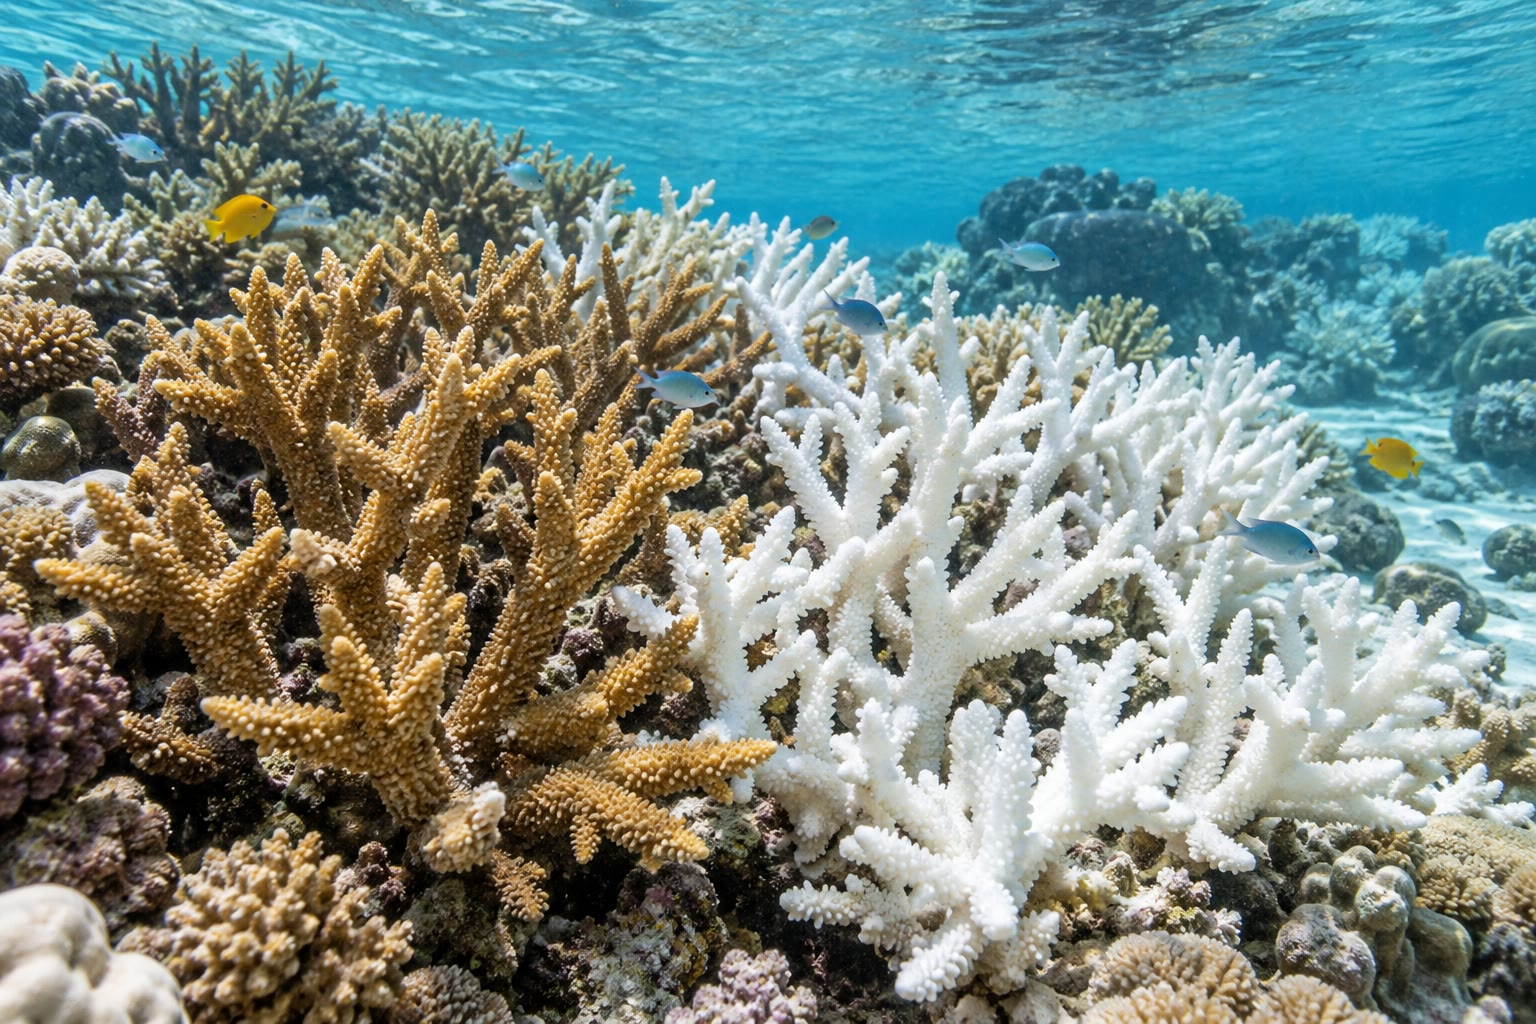
\includegraphics[width=0.44\linewidth]{images/book4/ai/b4-27-coral-bleaching.jpg}\hspace{0.04\linewidth}
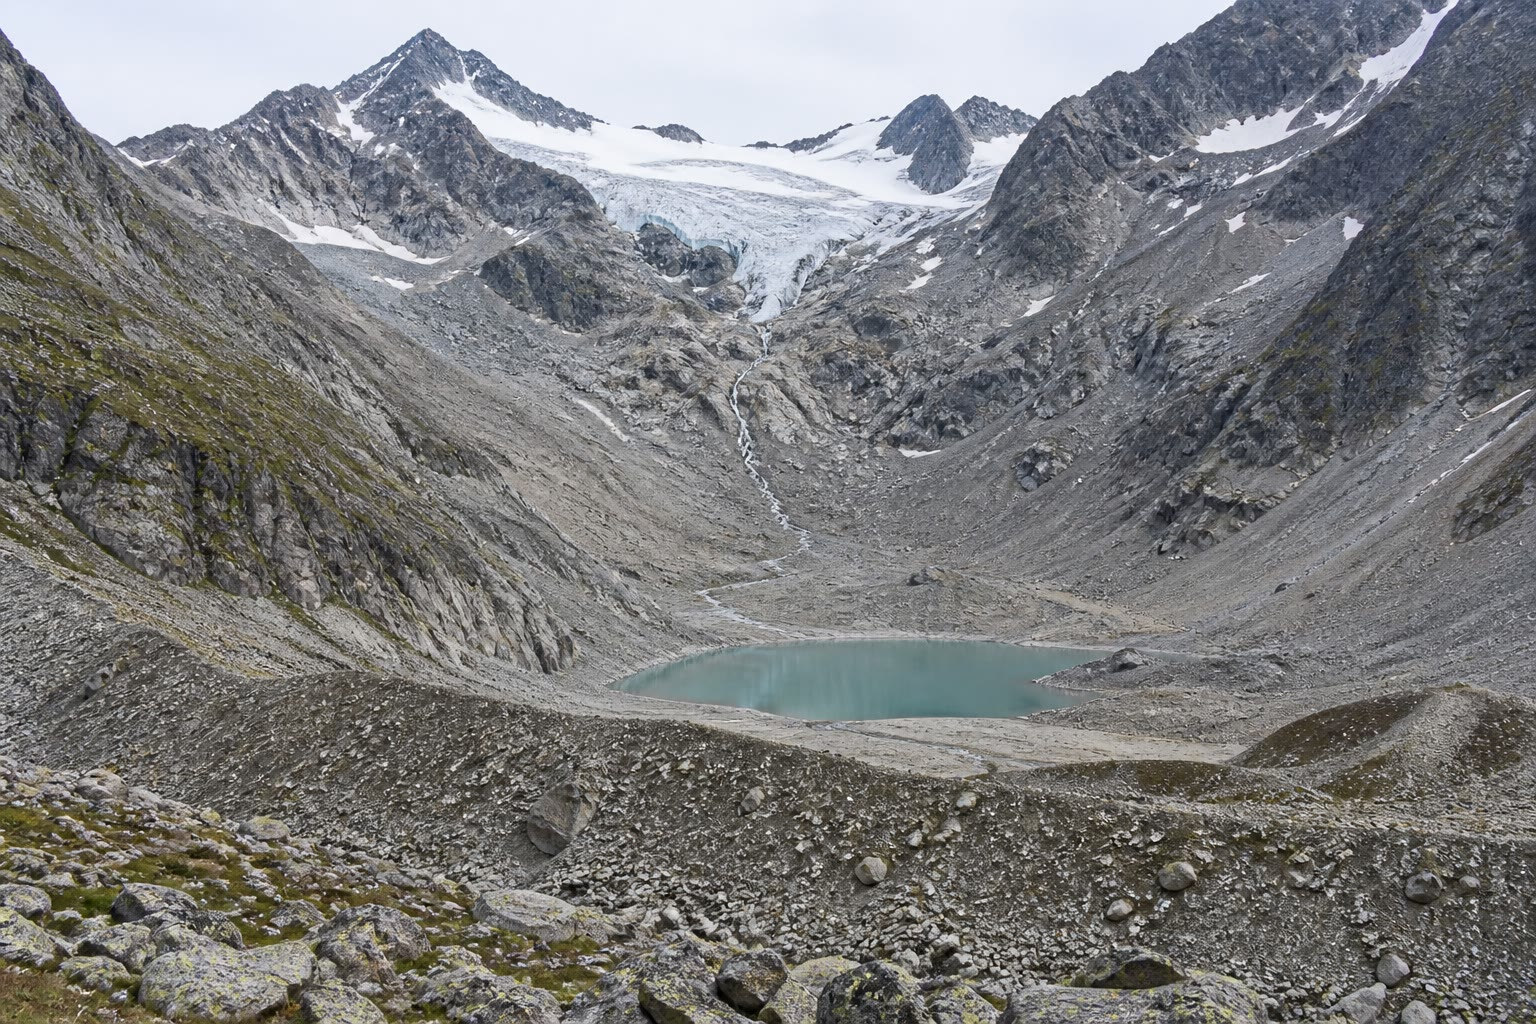
\includegraphics[width=0.44\linewidth]{images/book4/ai/b4-27-glacier-retreat.jpg}

{\small Twee thermometers. Links: een verbleekt rif, het witte skelet van het
koraal dat zichtbaar wordt door weefsel dat zijn algen kwijt is. Rechts: een
dalgletsjer die zich in zijn dal heeft teruggetrokken en kaal gesteente
achterlaat waar een eeuw geleden ijs lag.}
\end{omfigure}

\section{De balans: uitsterven en de schatting ervan}

\begin{theorem}[De soorten-oppervlakterelatie en de kosten van habitatverlies]\label{thm:b2:global-change:sar}
\index{soorten-oppervlakterelatie}\index{extinctiesnelheid}\index{habitatverlies}\index{extinctieschuld}
Het aantal soorten in een oppervlak $A$ groeit als een macht van het
oppervlak, $S = cA^{z}$, met $z \approx 0.25$ voor eilanden en
habitatfragmenten (een verdubbeling van het oppervlak voegt een vijfde meer
soorten toe; een honderd keer groter oppervlak geeft drie keer zoveel). Als een
habitat wordt teruggebracht tot een fractie $1 - h$ van zijn omvang, daalt het
aantal soorten dat het uiteindelijk kan herbergen tot $(1 - h)^{z}$ van het
oorspronkelijke: het verlies van de helft van het habitat kost \qty{16}{\%} van
zijn soorten, \qty{90}{\%} kost \qty{44}{\%}, en \qty{99}{\%} kost
\qty{68}{\%}. Het verlies is niet onmiddellijk --- de overlevenden in het
fragment houden het een tijd uit, een \emph{\omterm{thm:b2:global-change:sar}{extinctieschuld}} die over
decennia wordt afbetaald naarmate kleine populaties bezwijken aan de drift en
inteelt van \cref{ch:b2:population-genetics} --- en het is de basis van de
schatting dat de huidige \omterm{thm:b2:global-change:sar}{extinctiesnelheid} honderd tot duizend keer de
achtergrondsnelheid van het fossielenbestand is: ongeveer één soort op een
miljoen per jaar, tegenover de enkele duizenden per jaar, op zo'n tien miljoen,
die nu verloren gaan.
\end{theorem}
\begin{proof}
$S'/S = (A'/A)^{z} = (1 - h)^{z}$; met $z = 0.25$ is $0.5^{0.25} =
0.84$, $0.1^{0.25} = 0.56$, $0.01^{0.25} = 0.32$. De relatie
zelf is empirisch; haar exponent weerspiegelt op eilanden het evenwicht
tussen de immigratie van nieuwe soorten (die daalt naarmate het eiland
volloopt) en het uitsterven van aanwezige soorten (dat stijgt naarmate hun
populaties met het oppervlak krimpen), het evenwicht uit de theorie van
MacArthur en Wilson.
\end{proof}
\begin{proof}[Bewijsmateriaal]
De eilanden van de Krakatau-groep, gesteriliseerd door de uitbarsting van
1883, werden opnieuw gekoloniseerd door planten, vogels en insecten in een
successie die binnen vijftig jaar de soortenaantallen bereikte die uit hun
oppervlakte werden voorspeld; de mangrove-eilandjes die Simberloff en
Wilson in 1966 in Florida begasten, keerden binnen een jaar terug naar hun
oorspronkelijke soortenaantallen, met andere soorten. Het Atlantisch
woud van Brazilië, teruggebracht tot \qty{10}{\%} van zijn omvang, heeft de
fractie van zijn vogelsoorten die de relatie voorspelt verloren of bijna
verloren; en in elke groep die door de Internationale Unie voor Natuurbehoud is
beoordeeld, is een kwart tot een derde van de soorten bedreigd --- vogels
\qty{13}{\%}, zoogdieren \qty{27}{\%}, amfibieën \qty{41}{\%}, koralen
\qty{44}{\%} --- met \omterm{thm:b2:global-change:sar}{habitatverlies} als eerste oorzaak, en jacht,
\omterm{prop:b2:global-change:invasion}{invasieve soorten}, vervuiling en, steeds meer, het klimaat als de andere.
\end{proof}

\begin{omfigure}
\begin{tikzpicture}
\begin{loglogaxis}[
  width=0.68\linewidth, height=5.4cm,
  axis x line=bottom, axis y line=left,
  xmin=1, xmax=100000, ymin=5, ymax=200,
  xlabel={eilandoppervlakte (\unit{km^2})}, ylabel={soorten landvogels},
  xlabel style={font=\small, at={(axis description cs:0.5,-0.13)}, anchor=north},
  ylabel style={font=\small},
  tick label style={font=\small},
  clip=false,
]
\addplot[only marks, mark=*, mark size=2pt, omDef] coordinates {(1.5,9) (8,14) (35,22) (150,32) (400,37) (1200,52) (4000,70) (13000,92) (35000,125) (85000,160)};
\addplot[very thick, omThm, domain=1:100000, samples=2] {9*x^0.25};
\node[font=\scriptsize, omThm, anchor=north west, align=left] at (axis cs:2,120) {$S = 9A^{0.25}$: honderd keer\\ meer oppervlak, drie keer\\ zoveel soorten};
\end{loglogaxis}
\end{tikzpicture}

{\small De \omterm{thm:b2:global-change:sar}{soorten-oppervlakterelatie}, hier voor landvogels op eilanden
van een archipel: een rechte lijn met helling $z = 0.25$ op
logaritmische assen. Breng een habitat terug tot een tiende en het zal na
verloop van tijd weinig meer dan de helft van zijn soorten behouden.}
\end{omfigure}

\begin{proposition}[Invasies, diensten, en wat er te doen valt]\label{prop:b2:global-change:invasion}
\index{invasieve soort}\index{ecosysteemdiensten}\index{mitigatie}\index{netto nul}
Schepen, vliegtuigen en handel hebben duizenden soorten voorbij de barrières
gebracht die ze gescheiden hielden; de meeste vestigen zich niet, maar de
enkele die het wel doen --- het konijn in Australië, de driehoeksmossel in de
Grote Meren, de bruine nachtboomslang die Guam van zijn vogels ontdeed,
de chytridschimmel die negentig amfibiesoorten tot
uitsterven heeft gedreven --- verspreiden zich als een front dat met constante
snelheid oprukt, $c =
2\sqrt{rD}$ voor een populatie die groeit met snelheid $r$ en zich verspreidt
met diffusiecoëfficiënt $D$ (de muskusrat van Skellam, in 1905 bij
Praag uitgezet, breidde zich met \qty{11}{km} per jaar over Europa uit,
met de straal van zijn areaal als rechte lijn in de tijd). Daartegenover staat
wat de biosfeer doet voor haar ene lastige soort:
\omterm{def:b2:angiosperm-reproduction:pollination}{bestuiving} van drie kwart van de gewassen, waterzuivering, bescherming tegen
overstromingen, het binden van stikstof en het maken van \omterm{def:b2:living-soil:soil}{bodem}, visserij,
de koolstof die in bossen en \omterm{def:b2:living-soil:soil}{bodems} zit --- \emph{ecosysteemdiensten}
die, waar er een prijs op kan worden geplakt, meer waard worden geschat dan het
economische product van de wereld. Wat er te doen valt, volgt uit de getallen.
De opwarming stopt wanneer de netto-uitstoot stopt, en niet eerder: de
boxmodellen van \cref{ch:b2:biogeochemical-cycles} laten geen andere
lezing van \emph{\omterm{prop:b2:global-change:invasion}{netto nul}} toe. Land kan binnen grenzen helpen --- een
gigaton koolstof per jaar uit herbebossing en \omterm{def:b2:living-soil:soil}{bodems} gedurende enkele
decennia, tegenover tien uit fossiele brandstoffen --- en soorten kunnen worden
geholpen te verhuizen, of worden bewaard in reservaten die groot en verbonden
genoeg zijn om te voorkomen dat de \omterm{thm:b2:global-change:sar}{soorten-oppervlakterelatie} en de drift van
kleine populaties ze uitroeien. De gereedschappen zijn die van dit boek: de
\omterm{def:b2:population-genetics:frequencies}{populatiegenetica} van het reservaat, de concurrentie van de
indringer, de fenologie van het gewas, het budget van de \omterm{def:b2:living-soil:soil}{bodem}.
\end{proposition}

\begin{example}[Drie toekomsten]\label{ex:b2:global-change:scenarios}
Een uitstoot die tot 2100 op \qty{10}{GtC} per jaar blijft, voegt \qty{800}{GtC}
toe aan de \qty{700}{} die al zijn uitgestoten: $1.65\times 1.5 =
\qty{2.5}{\celsius}$ tegen het eind van de eeuw, en nog stijgend. Een uitstoot
die tegen 2070 tot nul daalt, voegt ongeveer \qty{250}{GtC} toe: \qty{1.6}{\celsius},
en daarna vlak. Eerst de uitstoot verdubbelen, zoals de eerste decennia van de
eeuw deden, geeft \qty{4}{\celsius} of meer. De arealen van de
gematigde zone verschuiven in het eerste geval \qty{200}{km} voorbij die van vandaag
en in het tweede \qty{60}{km}; de lente komt vijfentwintig
dagen vroeger, of zes; de pH aan het oppervlak bereikt $7.8$, of blijft rond
$8.0$; en de schattingen van het uitsterven, die van habitat en
opwarming samen afhangen, lopen van een tiende tot een derde van de soorten. Het
verschil tussen de toekomsten is het cumulatieve oppervlak onder één
curve, en dat is de som van beslissingen die nog niet zijn genomen.
\end{example}

\section{Opgaven}

\begin{exercise}[$\star$]\label{exo:b2:global-change:1}
Formuleer het verband tussen opwarming en \omterm{prop:b2:global-change:tcre}{cumulatieve uitstoot}, en
bereken de opwarming voor een \omterm{prop:b2:global-change:tcre}{cumulatieve uitstoot} van 700, 1000 en
\qty{2000}{GtC}.
\end{exercise}

\begin{exercise}[$\star$]\label{exo:b2:global-change:2}
Definieer graaddagen en \omterm{thm:b2:global-change:phenology}{fenologische ontkoppeling}, met de vliegenvanger
als voorbeeld.
\end{exercise}

\begin{exercise}[$\star$]\label{exo:b2:global-change:3}
Hoe ver verschuiven isothermen per graad opwarming bergop en naar de pool,
en waarom kan een soort van de bergtop niet volgen?
\end{exercise}

\begin{exercise}[$\star$]\label{exo:b2:global-change:4}
Leg in drie zinnen uit waarom het toevoegen van \ensuremath{\mathrm{CO_2}} aan de zee
haar pH en haar carbonaat verlaagt, en welke organismen erdoor worden getroffen.
\end{exercise}

\begin{exercise}[$\star\star$]\label{exo:b2:global-change:5}
Bereken het resterende koolstofbudget voor \qty{1.5}{\celsius} en voor
\qty{2}{\celsius} met $\lambda = \qty{1.65}{\celsius}$ per
\qty{1000}{GtC} en \qty{700}{GtC} al uitgestoten; reken beide om in
jaren bij \qty{10}{GtC/yr}.
\end{exercise}

\begin{exercise}[$\star\star$]\label{exo:b2:global-change:6}
De lente warmt op met $b = \qty{0.12}{\celsius}$ per dag vanaf een basis van
\qty{5}{\celsius}; een nachtvlinder heeft $K = 150$ graaddagen nodig. Bereken
het aantal dagen van het overschrijden van de basis tot het uitkomen, en de
vervroeging bij een opwarming van \qty{1.5}{\celsius}.
\end{exercise}

\begin{exercise}[$\star\star$]\label{exo:b2:global-change:7}
Het areaal van een plant beslaat \qtyrange{800}{1400}{m} op een berg van
\qty{1800}{m} hoog waarvan het oppervlak per \qty{300}{m} hoogte halveert.
Waar ligt de band na \qty{3}{\celsius} opwarming, en hoeveel oppervlak is hij
kwijt? En na \qty{5}{\celsius}?
\end{exercise}

\begin{exercise}[$\star\star$]\label{exo:b2:global-change:8}
Bereken de pH aan het oppervlak en de stijging van de waterstofionconcentratie
bij 560, 800 en \qty{1000}{ppm}, uit $\mathrm{pH} = 8.2 -
0.9\log_{10}(p/280)$.
\end{exercise}

\begin{exercise}[$\star\star$]\label{exo:b2:global-change:9}
Welke fractie van de soorten gaat met $z = 0.25$ uiteindelijk verloren wanneer
\qty{70}{\%}, \qty{95}{\%} en \qty{99.9}{\%} van een habitat wordt
vernietigd? Waarom is het onmiddellijke verlies kleiner?
\end{exercise}

\begin{exercise}[$\star\star\star$]\label{exo:b2:global-change:10}
Een indringer groeit met $r = 0.7$ per jaar en verspreidt zich met $D =
\qty{20}{km^2/yr}$. Bereken de snelheid van zijn front en de tijd om een
land van \qty{1000}{km} breed over te steken. Wat halveert de snelheid: $r$
halveren of $D$ halveren?
\end{exercise}

\begin{exercise}[$\star\star\star$]\label{exo:b2:global-change:11}
De achtergrondsnelheid van uitsterven is 1 per miljoen soortjaren en
er zijn 8 miljoen soorten. Bereken het verwachte aantal uitstervingen per
jaar en per eeuw bij de achtergrondsnelheid, en bij 1000 keer de achtergrond.
Vergelijk met de tienduizend gedocumenteerde uitstervingen van de afgelopen
eeuw en geef commentaar op het verschil.
\end{exercise}

\begin{exercise}[$\star\star\star$]\label{exo:b2:global-change:12}
``De opwarming stopt wanneer de netto-uitstoot stopt.'' Verantwoord dit met het
\omterm{thm:b2:biogeochemical-cycles:box}{boxmodel} van de atmosfeer en de evenredigheid van de opwarming met de
\omterm{prop:b2:global-change:tcre}{cumulatieve uitstoot}, en zeg wat er aan het argument ontbreekt.
\end{exercise}

\section{Vraagstuk: de biosfeer in 2100}

\begin{problem}[{Weekendvraagstuk --- twee uitstootpaden doorgetrokken
tot 2100: de opwarming van elk pad, de lente die het oplevert, de afstand
die zijn isothermen afleggen, het zuur dat het in de zee brengt en de soorten
die het een bos kost, met als besluit de twee opwarmingen, de twee pH-waarden
en de fractie verloren soorten}]
\label{pb:b2:global-change:1}
Gegevens. $\lambda = \qty{1.65}{\celsius}$ per \qty{1000}{GtC};
\qty{700}{GtC} uitgestoten tegen 2020 (opwarming \qty{1.2}{\celsius}). Pad
A: \qty{10}{GtC/yr} constant tot 2100. Pad B: lineair dalend tot
nul in 2070. De lente warmt op met $b = \qty{0.1}{\celsius}$ per dag
boven een basis van \qty{5}{\celsius}; een boom heeft $K = 200$
graaddagen nodig om blad te krijgen, en een trekvogel komt op een vaste datum
aan, in 2020 20 dagen na de bladontplooiing van de boom. Verticale gradiënt
\qty{6.5}{\celsius/km}; gradiënt met de breedtegraad \qty{0.65}{\celsius}
per \qty{100}{km}. Oceaan: $\mathrm{pH} = 8.2 - 0.9\log_{10}(p/280)$;
\ensuremath{\mathrm{CO_2}} in 2100: \qty{600}{ppm} op pad A, \qty{420}{ppm} op pad B.
Een bosgebied van \qty{e5}{km^2} met 400 boomsoorten, $z = 0.25$,
verliest tegen 2100 op pad A \qty{60}{\%} van zijn oppervlak aan ontbossing en
op pad B \qty{20}{\%}.

\medskip
\noindent\textbf{Deel I --- Opwarming.}
\begin{enumerate}
  \item Bereken de \omterm{prop:b2:global-change:tcre}{cumulatieve uitstoot} in 2100 op elk pad.
  \item Bereken de opwarming in 2100 op elk pad.
  \item Bereken de opwarming in 2050 op elk pad.
  \item Wat is het opwarmingstempo per decennium op pad A? Vergelijk met
        de waargenomen \qty{0.2}{\celsius} per decennium.
  \item Stopt de opwarming op pad B in 2070? Waarom, volgens de
        evenredigheid?
  \item Welke \omterm{prop:b2:global-change:tcre}{cumulatieve uitstoot} komt overeen met \qty{2}{\celsius},
        en in welk jaar overschrijdt pad A die?
\end{enumerate}

\medskip
\noindent\textbf{Deel II --- Lente.}
\begin{enumerate}[resume]
  \item Bereken het aantal dagen van het overschrijden van de basis tot de
        bladontplooiing in 2020.
  \item Bereken de vervroeging van de bladontplooiing ten opzichte van 2020 in
        2100 op elk pad (opwarming ten opzichte van 2020).
  \item De aankomstdatum van de vogel verandert niet. Bereken de kloof
        tussen bladontplooiing en aankomst op elk pad in 2100.
  \item De rupsen die de vogel nodig heeft, pieken 15 dagen na de
        bladontplooiing en blijven 10 dagen. Op welk pad vindt de vogel ze
        nog?
  \item Stel dat de vogel in plaats daarvan \qty{3}{d} per graad vervroegt.
        Bereken de kloof op pad A opnieuw.
  \item Zeg in één zin waarom de ontkoppeling, en niet de opwarming
        zelf, de vogel bedreigt.
\end{enumerate}

\medskip
\noindent\textbf{Deel III --- Arealen.}
\begin{enumerate}[resume]
  \item Bereken de verschuiving van de isothermen in hoogte en breedte
        op elk pad, ten opzichte van 2020.
  \item Een boomsoort verspreidt zich \qty{100}{m} per jaar. Kan ze de
        isothermen naar de pool volgen op pad A? Op pad B?
  \item Een soort bezet \qtyrange{1500}{1800}{m} op een berg van
        \qty{2000}{m}. Waar ligt haar band op pad A in 2100, en wat gebeurt er?
  \item Het oppervlak van de berg halveert per \qty{300}{m}. Bereken de
        oppervlaktefactor die die soort op pad B verliest.
  \item Een zeevis volgt isothermen met \qty{30}{km} per decennium.
        Is dat genoeg op pad A?
  \item Leg uit waarom de ondergrens van een areaal terugtrekt, zelfs waar
        de soort de warmte zou kunnen verdragen.
\end{enumerate}

\medskip
\noindent\textbf{Deel IV --- Zee en bos.}
\begin{enumerate}[resume]
  \item Bereken de pH aan het oppervlak in 2100 op elk pad, en de stijging
        van de waterstofionconcentratie sinds 1750.
  \item De \omterm{thm:b2:global-change:acid}{verzadigingstoestand} $\Omega$ van het tropische oppervlaktewater was
        in 1750 gelijk aan 4 en daalt als $[\ensuremath{\mathrm{H^{+}}}]^{-1}$. Bereken hem in 2100
        op elk pad en zeg wat dat voor koraal betekent.
  \item Bereken het aantal boomsoorten dat het bosgebied op elk pad
        uiteindelijk kan herbergen, en het aantal verloren soorten.
  \item Opwarming voegt verliezen toe: stel dat elke graad boven 2020 nog eens
        \qty{5}{\%} van de overlevende soorten wegneemt. Bereken opnieuw
        de soorten die op elk pad overblijven.
  \item Geef de fractie van de 400 soorten die op elk pad verloren gaat.
  \item Welke van de twee oorzaken, ontbossing of opwarming, overheerst op
        elk pad?
  \item Formuleer het resultaat: de opwarming, de pH en de fractie
        verloren boomsoorten in 2100 op elk pad.
\end{enumerate}
\end{problem}
